\thispagestyle{fancy}
\vspace*{\fill}
\subsection{Tela comando slotter}
 Esta tela é acessada pelo botão "\textgreater" no menu superior esquerdo da tela de comando slotter, pelo botão "\textless{}" no menu superior esquerdo da tela comando dobra, pelo botão "PRF" em qualquer tela de comando e pelo botão comando da tela ajustes perfuradora.
\begin{figure}[h]
  \centering
  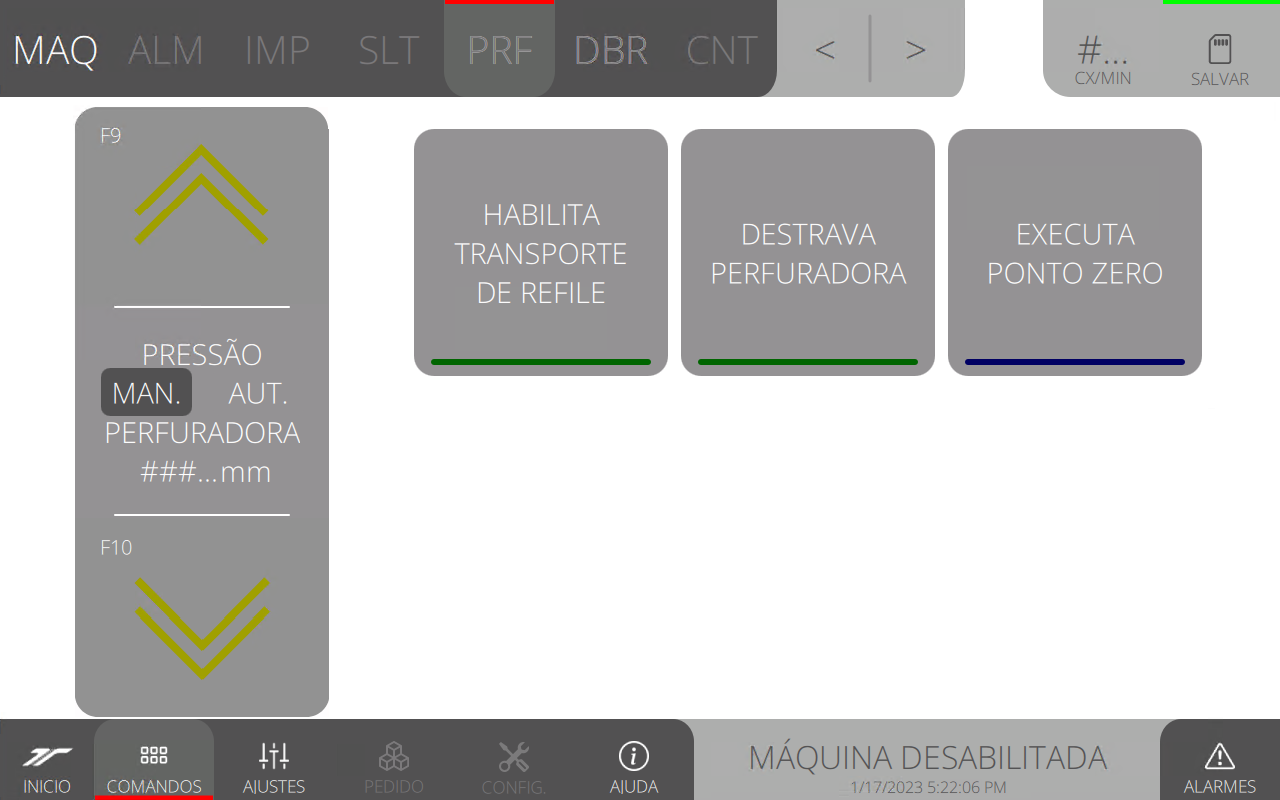
\includegraphics[width=576px,height=360px]{src/imagesFlexo/06-drilling/commands/e-Tela-Principal.png}
  \caption{ver depois.}
   \label{}
\end{figure}

\newpage
\thispagestyle{fancy}
\vspace*{\fill}
\subsubsection{\small{Ajuste pressão porta manta}}
\begin{figure}[h]
  \centering
  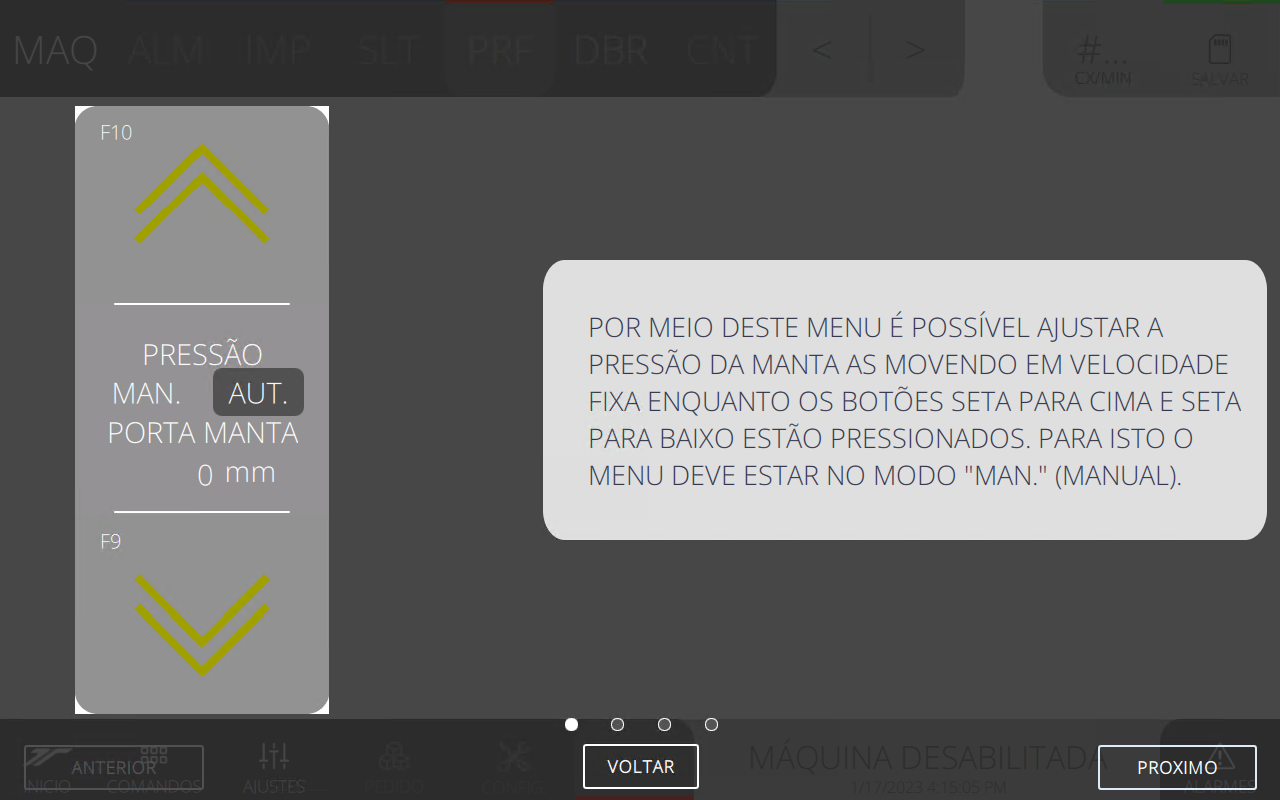
\includegraphics[width=576px,height=360px]{src/imagesFlexo/06-drilling/commands/e-1.png}
  \caption{ver depois.}
   \label{}
\end{figure}
\vspace*{\fill}

\newpage
\thispagestyle{fancy}
\vspace*{\fill}
\subsubsection{\small{Executa ponto zero}}
\begin{figure}[h]
  \centering
  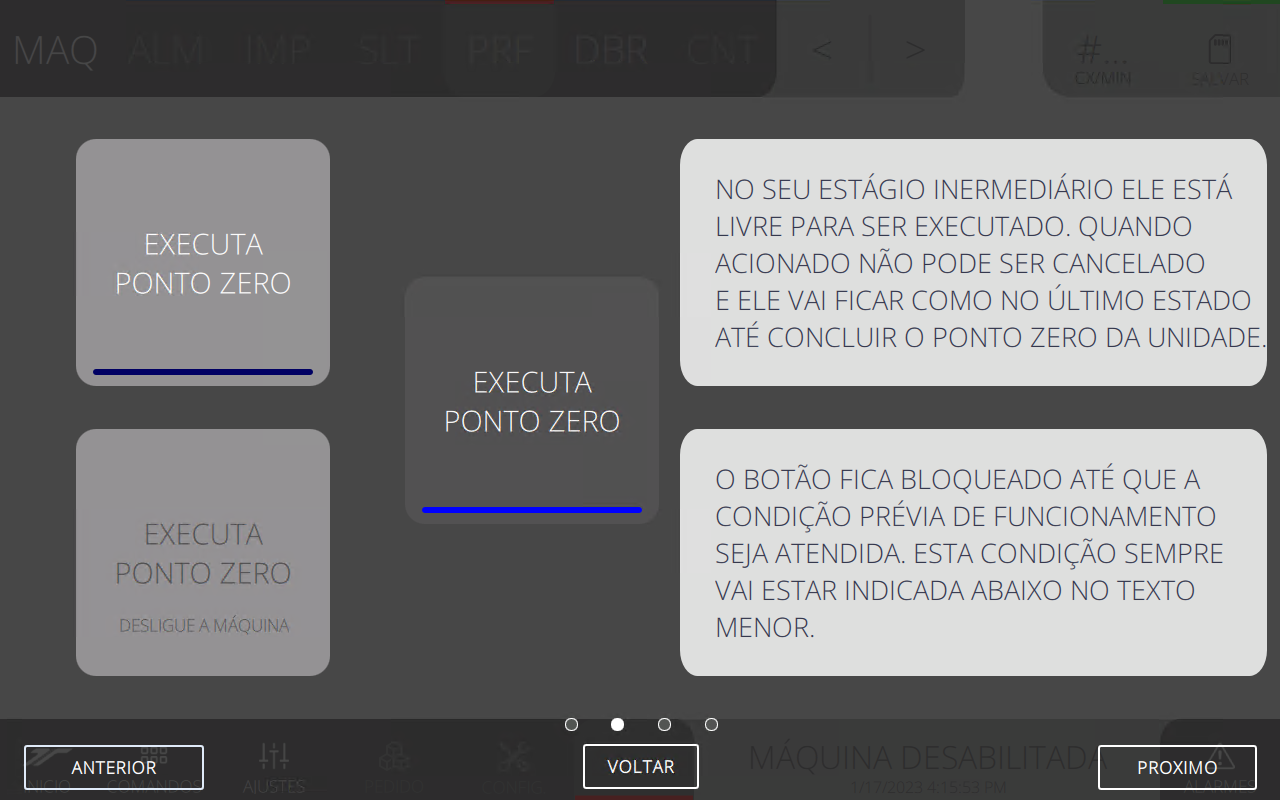
\includegraphics[width=576px,height=360px]{src/imagesFlexo/06-drilling/commands/e-2.png}
  \caption{ver depois.}
   \label{}
\end{figure}
\vspace*{\fill}

\newpage
\thispagestyle{fancy}
\vspace*{\fill}
\subsubsection{\small{Habilita transporte de refile}}
\begin{figure}[h]
  \centering
  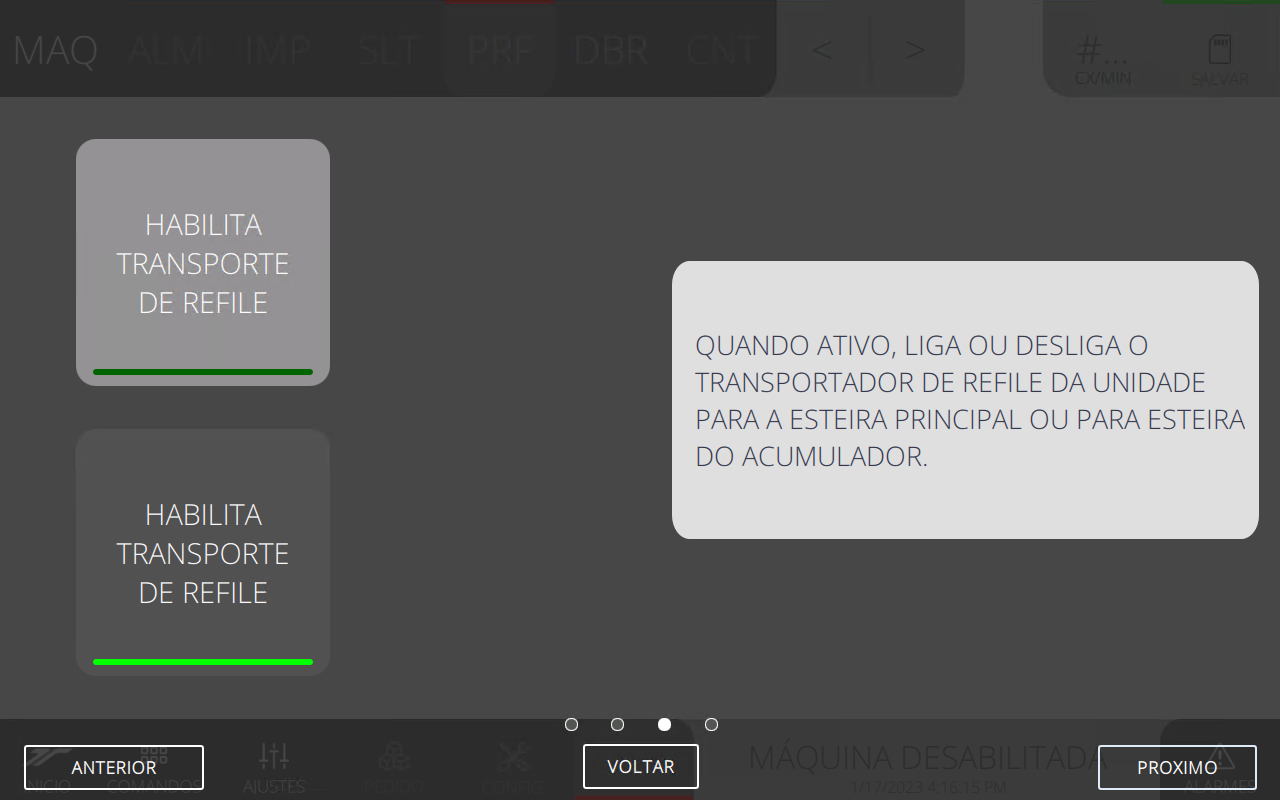
\includegraphics[width=576px,height=360px]{src/imagesFlexo/06-drilling/commands/e-3.png}
  \caption{ver depois.}
   \label{}
\end{figure}
\vspace*{\fill}

\newpage
\thispagestyle{fancy}
\vspace*{\fill}
\subsubsection{\small{Trava perfuradora}}
\begin{figure}[h]
  \centering
  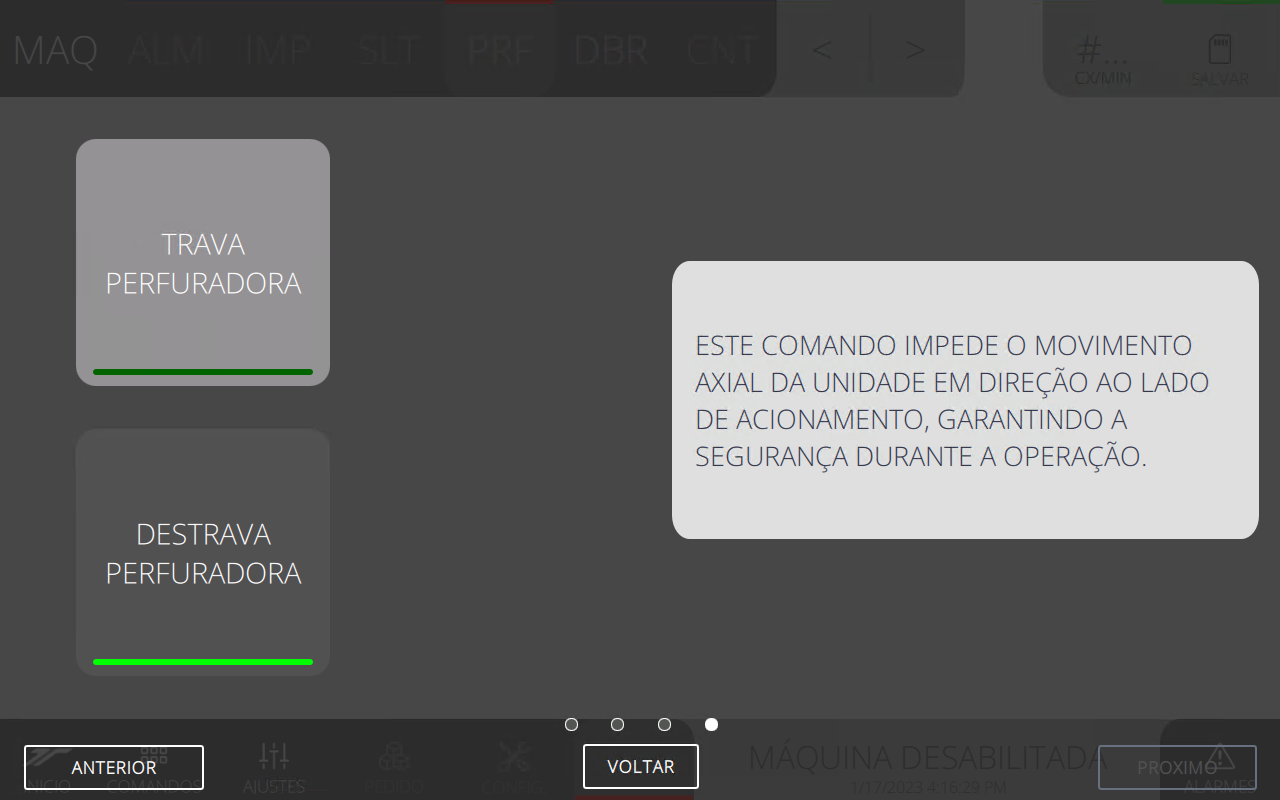
\includegraphics[width=576px,height=360px]{src/imagesFlexo/06-drilling/commands/e-4.png}
  \caption{ver depois.}
   \label{}
\end{figure}
\vspace*{\fill}
